\documentclass[diploma]{nanolab2015}

\usepackage{tikz}
\usepackage{tkz-graph}
\usepackage{float}
\usepackage{subfigure}
\usepackage{booktabs}
\usepackage{dcolumn}
\usepackage[flushleft]{threeparttable}
\usepackage{makecell}
\usepackage{enumitem}
\usepackage{xparse}
\usepackage{svg}
\newcounter{descriptcount}
\NewDocumentEnvironment{enumdescript}{O{}}{%
    \setcounter{descriptcount}{0}%
    \renewcommand*\descriptionlabel[1]{%
      \stepcounter{descriptcount}%
      \normalfont\bfseries ##1%
    }%
    \description%
  }%
  {\enddescription}



\DeclareMathOperator{\Attention}{Attention}
\DeclareMathOperator{\softmax}{softmax}
\DeclareMathOperator{\ReLU}{ReLU}
\DeclareMathOperator{\MSE}{MSE}
\DeclareMathOperator{\AdamW}{AdamW}


\begin{document}
\begin{titlepage}
  \begin{center}
    ФЕДЕРАЛЬНОЕ ГОСУДАРСТВЕННОЕ БЮДЖЕТНОЕ ОБРАЗОВАТЕЛЬНОЕ УЧРЕЖДЕНИЕ ВЫСШЕГО ОБРАЗОВАНИЯ

    <<МОСКОВСКИЙ ГОСУДАРСТВЕННЫЙ УНИВЕРСИТЕТ

    имени М.В.ЛОМОНОСОВА>>

    \vspace{0.7cm}

    МЕХАНИКО-МАТЕМАТИЧЕСКИЙ ФАКУЛЬТЕТ

    \vspace{0.7cm}

    КАФЕДРА Математической теории интеллектуальных систем 

    \vspace{3cm}

    ВЫПУСКНАЯ КВАЛИФИКАЦИОННАЯ РАБОТА
  
    (ДИПЛОМНАЯ РАБОТА)
  
    специалиста

    \vspace{0.7cm}

    \textbf{Использование графовых нейронных сетей в задачах информационного поиска для построения кликовой модели}

  \end{center}

  \vspace{2cm}

  \hfill
  \begin{minipage}{0.5\textwidth}
    Выполнил студент

    631

    Зенин Виктор Олегович

    \vspace{1cm}

    \underline{\hspace{4cm}}

    подпись студента

    \vspace{0.5cm}

    Научный руководитель:

    к.ф.-м.н., н.с.

    Половников Владимир Сергеевич

    \vspace{1cm}

    \underline{\hspace{4cm}}

    подпись научного руководителя
 \end{minipage}

  \vfill

  \begin{center}
    \large Москва

    \the\year
  \end{center}

\end{titlepage}

\setcounter{page}{3}
\clearpage
\tableofcontents{}  % оглавление
\clearpage
\chapter{Введение}
Информационные системы занимают центральное место в обработке больших объемов данных. С увеличением количества информации важно разрабатывать методы поиска, которые обеспечат пользователям быстрое нахождение нужной информации. Одним из важных источников данных являются действия пользователей при поиске и работе с найденной информацией. Исследуя подобные данные можно извлекать из них различные признаки, способные улучшать качество поисковой системы и лучше удовлетворять потребности пользователя.

Одним из способов работы с такими данными являются кликовые модели, которые анализируют имеющуюся историю взаимодействия пользователей с результатами поисковой выдачи и помогают лучше понять, какие из показанных документов были более или менее полезны. Традиционные подходы к построению кликовых моделей включают в себя различные вероятностные методы, однако с развитием технологий машинного обучения все более актуальным становятся нейросетевые методы, обладающие в некоторых задачах высокой обобщающей способностью, позволяющей эффективно обрабатывать и анализировать сложные и многомерные данные.

Актуальность данной темы обусловлена как практическими потребностями, так и научным интересом. С одной стороны, улучшение алгоритмов информационного поиска напрямую влияет на качество пользовательского опыта и способность поисковых систем решать свою главную задачу по нахождению релевантного контента. С другой стороны, исследование нейросетевых методов в контексте кликовых моделей открывает новые горизонты в области машинного обучения и обработки больших данных.

Целью данной работы является изучение современных нейросетевых методов построения кликовых моделей и их применения в задачах информационного поиска. В работе будут рассмотрены как теоретические аспекты разработки таких моделей, так и практические примеры их внедрения и оценки эффективности. Мы проанализируем существующие подходы, выявим их преимущества и недостатки, а также предложим алгоритм, позволяющий сократить время обучения графовой нейронной сети без потери качества.

Также мы предложим новую классическую кликовую модель VSDBN, которая будет использовать время просмотра в качестве поведенческого сигнала и может быть применима в тех областях поиска, где это наиболее актуально, например, в поиске видеороликов. 
\newpage
\section{Основные понятия и терминология}
\subsection{Поисковый запрос}
Поисковый запрос $q$ -- это текстовая строка, состоящая из ключевых слов, с которыми пользователь обращается к поисковой системе с целью удовлетворить свою информационную потребность. Основная задача информационного поиска это удовлетворение информационной потребности пользователя, которая выражена в составленном им запросе, посредством предоставления ему поисковой выдачи.

\subsection{Поисковая выдача}

Поисковая выдача по запросу $i$ -- это набор результатов $D_i$, которые поисковая система представляет пользователю в ответ на его поисковый запрос. Результаты включают ссылки на различные документы $(d_{i,1}, \dots, d_{i, M})$, которые поисковая система считает релевантными запросу пользователя.

Страницу результатов поиска, которую пользователь видит после ввода поискового запроса, принято называть серп, от SERP -- Search Engine Results Page. Серп обычно включает органические результаты (неоплаченные ссылки), платные результаты (рекламные ссылки), а также другие элементы, такие как изображения, видео, карты и фрагменты с ответами на вопросы.

\subsection{Пользовательская сессия}

Пользовательская сессия $S$ в контексте информационного поиска представляет собой последовательность взаимодействий пользователя с поисковой системой в течение определенного периода времени. В зависимости от контекста и целей анализа, можно выделить два типа сессий: сессии в широком смысле и сессии в узком смысле. Сессии в широком смысле будем обозначать $S$, сессии в узком смысле $s$, а множество всех сессий -- $\mathcal{S}$.

Сессия в широком смысле включает все действия пользователя, связанные с поиском информации, начиная с ввода первого поискового запроса $q_1$ и заканчивая завершением активности или истечением времени неактивности. В эту сессию входят все последующие перезапросы, изменения поисковых фраз, составляющие последовательность запросов $Q = \{q_i\}_{i=1}^N$, переходы по ссылкам, возвращения на страницу поиска, а также клики $C = \{c_{i,j}\}$ на результаты поиска, где $i$ -- порядковый номер запроса, к которому относятся клики по документам на позиции $j$. Клик кодируется бинарно $c_{i,j} \in \{0, 1\}$ -- 1 в случае клика и 0 иначе.

Каждая пользовательская сессия является тройкой: $(Q, C, D)$. По необходимости, для обозначения конкретной сессии из набора будем использовать индекс $k$. В случае сессий в широком смысле $\mathcal{S} = \{S_k\}_{k=1}^K$ каждой сессии $S_k$ соответствует тройка $(Q_{k} = \{q_{i,k}\}, C = \{c_{i,j,k}\}, D = \{d_{i,j,k}\})$. В случае сессий в узком смысле индекс $i$ можно опустить и писать соответственно $\mathcal{S} = \{s_k\}_{k=1}^K$ и $(Q_{k} = \{q_{k}\}, C = \{c_{j,k}\}, D = \{d_{j,k}\})$.

Сессия в узком смысле ограничивается взаимодействием пользователя в рамках одного конкретного поискового запроса $q$. В нее входят действия, связанные только с этим запросом.

Не трудно заметить, что сессия в широком смысле является последовательностью сессий в узком смысле и может быть на них разбита. Обратное же не верно, поскольку заданные в разное время пользовательские запросы могут не относится к удовлетворению его конкретной информационной потребности.

Действия пользователя зависят от типа показанного контента и не ограничиваются только кликами. Каждый такой тип принято называть вертикалью поиска, а контент -- принадлежащим соответствующей вертикали. У каждой поисковой вертикали могу быть специфические для нее особенности, например если поисковая система показала видео в серпе, то гораздо важнее знать, сколько времени пользовать его смотрел или досмотрел ли до конца.

\subsection{Релевантность}
Релевантность обозначает степень соответствия между поисковым запросом пользователя и предоставленными поисковой системой результатами. Чем выше степень соответствия между запросом и результатами, тем более релевантными считаются эти результаты для пользователя.

Иными словами, релевантность показывает, насколько хорошо результат поиска отвечает на запрос пользователя и удовлетворяет его информационные потребности. Это не только соответствие ключевым словам в запросе и содержанию документа, но и более общие факторы, такие как тематика, контекст и цель запроса.

Поисковая выдача формируется посредством работы алгоритма ранжирования, который анализирует признаки документов и упорядочивает их.

Для оценки релевантности составляется специальная инструкция, по которой эксперты, -- асессоры, -- оценивают пары запрос-документ и выставляют каждой из них оценку -- как правило это неотрицательное целое число.

Когда каждой паре запрос-документ сопоставлена такая численная оценка релеватности документа по этому запросу $rel$, можно оценить качество алгоритма ранжирования вычислив $DCG$ -- Discounted Cumulative Gain по формулам:
\begin{align}
    DCG@N = \sum_{j=1}^{N} \frac{rel_j}{log_2(j+1)} \label{dcg}
\end{align}
или
\begin{align}
    DCG_{exp}@N = \sum_{j=1}^{N} \frac{2^{rel_j} - 1}{log_2(j+1)} \label{dcg:exp}
\end{align}
где $N$ -- количество документов в выдаче, $j$ - позиция документа и $rel_j$ -- его релевантность. Можно заметить, что релевантные документы, оказавшиеся на последних позициях, дают малый вклад. Также как малый вклад дают и нерелевантные документы, оказавшиеся на первых позициях.

Существует способ нормализации $DCG$, приводящий её значения в диапазон от 0 до 1, заключающийся в вычислении $IDCG$ -- Ideal DCG. $IDCG$ это максимальное значение $DCG$ для данного запроса, но используя те же самые документы. Формула идентична (\ref{dcg}) или (\ref{dcg:exp}) (в зависимости от выбранной версии), за исключением того, что все документы должны быть отсортированы в порядке убывания их релевантности, т.е. при $j=1$ получается максимальная оценка релевантности из набора.
После чего нормализованный $DCG$, называющийся $nDCG$, вычисляется как отношение $DCG$ к соответствующему ему $IDCG$. Поскольку так оценивается выдача по одному запросу, для оценки по группе запросов берётся среднее арифметическое.

\subsection{Кликовая модель}
Кликовая модель в классическом понимании -- это статистическая модель, которая предсказывает вероятность того, что пользователь совершит клик -- $\mathcal{P}_{i,j} = P(c_{i,j} = 1)$ по определенному результату в поисковой выдаче, основываясь на исторических данных о кликах пользователей.

В отличии от других областей, например рекомендательных технологий, в поиске ключевым элементом является запрос и пользовательские сессии агрегируются по нему.

\subsection{Позиционная предвзятость}
Позиционная предвзятость -- это явление, при котором вероятность клика на определенный результат поисковой выдачи зависит не только от релевантности документа, но и от позиции этого документа в списке результатов. Результаты, которые находятся выше на странице выдачи, получают больше кликов независимо от их фактической релевантности, поскольку пользователи склонны кликать на первые несколько ссылок, не анализируя их подробно.


\subsection{Сравнение качества кликовых моделей}
Качество кликовых моделей можно оценивать комплексно с качеством поискового движка в целом, используя описанную метрику релевантности $DCG$. Однако, если требуется сравнить две модели между собой на одном и том же наборе данных, то для этого подходит перплексия:

\begin{align}
    PPL@j = 2^{-\frac{1}{N}\sum_{i=1}^{N} \left[c_{i,j}\log\mathcal{P}_{i,j} + (1 - c_{i,j})\log(1 - \mathcal{P}_{i,j})\right]}
\end{align}

где $N$ -- количество запросов, $c$ -- метка фактически совершенного клика, а $\mathcal{P}$ -- предсказанная вероятность клика по документу на позиции $j$ по $i$-тому запросу.

Для оценки по всему серпу перплексия усредняется по каждой позиции:

\begin{align}
    PPL = \frac{1}{M} \cdot \sum_{j=1}^{M} PPL@j
\end{align}

Чем ниже перплексия, тем лучше алгоритм предсказывает тестовые данные. Чем выше, тем соответственно он хуже понимает зависимости в тренировочных данных, либо же данные разнородны. Поэтому перплексию принято использовать для сравнения нескольких алгоритмов или моделей машинного обучения на одинаковых наборах данных.

\section{Традиционные методы построения кликовых моделей}
В данном разделе мы последовательно рассмотрим некоторые методы, двигаясь от более простых к более сложным и каждый последующий метод будет учитывать недостатки предыдущего.
\subsection{CTR}
CTR (Click-Through Rate) — это метрика, используемая для измерения эффективности рекламы, поисковых результатов и других элементов, привлекающих клики. % метрика плохое слово, мы математики и это может сбить с толку

CTR рассчитывается как отношение количества кликов на определенный элемент (например, рекламное объявление или результат поиска) к количеству его показов. Формула для расчета CTR выглядит следующим образом:
\begin{align}
    CTR = \frac{clicks}{imps},
\end{align}
где $clicks = \sum_{i,j} c_{i,j} \cdot E_{i,j}$ -- количество кликов по документам $d_{i,j}$, которые пользователь видел ($E_{i,j}=1$) и $imps = \sum_{i,j}E_{i,j}$ -- количество показов этих документов пользователям в целом. Важно уточнить, что подразумевается под показом: пусть поисковый движок демонстрирует на странице 10 документов выдачи, но устройство пользователя, в самом простом примере, не позволяет отобразить их все сразу. Это значит, что, например, документ на позиции $j=10$ не виден $E_{i,10} = 0$ и пользователь априори не может на него кликнуть. Такие скрытые от пользователя документы не учитываются при вычислении $CTR$. То как пользователь обращает внимание на документы будет следовать некоторым гипотезам.

Для использования этой метрики в поиске важно, чтобы клики и показы документов происходили в рамках одного запроса. Таким образом, высокий CTR документа указывает на то, что пользователи чаще кликают по нему в контексте данного запроса, что предполагает его высокую релевантность и полезность. CTR может использоваться как дополнительный фактор в алгоритме ранжирования поисково движка, который, при прочих равных, стремился бы продвигать документы с высокой кликабельностью выше в выдаче.

Для сессий в широком смысле в качестве такого запроса можно использовать самый первый, исходя из предположения, что пользователь совершает перезапросы с целью уточнить первоначальный и найти в конечном итоге то, что у него не получилось найти с первого раза. Поскольку сессия в широком смысле содержит в себе несколько сессий в узком смысле, то CTR можно считать и по каждой такой сессии с уникальным запросом.

CTR обладает рядом существенных недостатков, среди самых важных можно выделить два: неустойчивость перед позиционной предвзятостью и злоупотреблением привлекательными заголовками. В первом случае высокий CTR будут получать документы на первых позициях в выдаче вне зависимости от их фактической релевантности. Во втором -- пользователя может заинтересовать непосредственно заголовок, в то время как сам документ покажется ему бесполезным и он быстро завершит его просмотр.

\subsection{ClickRank}
Данных метод применяется к сессиям в широком смысле и позволяет учесть время, которое пользователь проводит в документе.

Документами являются страницы в сети Интернет, переход на которых осуществляется кликом по странице в поисковой выдаче.
Пусть у нас имеется набор сессий в широком смысле $\mathcal{S} = \{S_k\}_{k=1}^K$. Каждой сессии из этого набора соответствует последовательность кликов $C_k$. Длиной сессии $n_k$ называется количество событий в $S_k$, в данном случае это количество кликов, т.е. $n_k = |C_k|$.

Документы из всех выдач внутри $S_k$ обозначим за $D_k = \{d_{k,p}\}_{p=1}^{|D_k|}$ -- их порядок в серпах не важен, поэтому мы можем рассматривать все документы в одном множестве опустив индексы $i,j$.
Стоит отметить, что $|C_k|$ в данном методе может быть больше $|D_k|$, поскольку пользователь может совершать клики в одни и те же документы многократно.

Каждый клик необходимо дополнить его индексом в последовательность кликов, а также можно избавиться от указания на принадлежность сессии в узком смысле, т.е. вместо индексов $i,j$ имеем: $C_k = (c_{k,p,r})$, где $r \in \{1, \dots, n_k\}$ и $p \in \{1, \dots, |D_k|\}$.

Каждой сессии $S_k$ установим в соответствие запрос $q_1 \in Q_k \in S_k$ и обозначим его $q_k$. Тогда локальный ClickRank \cite{clickrank} документа $d_{k,p}$ в сессии $S_k$ вычисляется следующим образом:
\begin{align}
    ClickRank(d_{k,p}, S_k) = \sum_{r=1}^{n_k} c_{k, p, r} \cdot w_r(r, n_k) \cdot w_t(k,p,r)
\end{align}

Весовая функция $w_r$ отвечает за порядок клика:
\begin{align}
    w_r(r, n_k) = \frac{2(n_k + 1 - r)}{n_k(n_k + 1)}
\end{align}

Функция является монотонно убывающей по $r$, что позволяет ей давать больший вес для кликнутых ранее документов. Поскольку пользователи кликают на документы из начала серпа раньше, данный метод не борется с позиционной предвзятостью. Однако он позволяет учитывать проводимое время посредством второй весовой функции $w_t$, которая отвечает за проведенное на странице время:
\begin{align}
    w_t(k,p,r) = (1 - e^{-\lambda_1 t_d(k,p,r)})e^{-\lambda_2 t_l(k,p,r)}
\end{align}

где $t_d(k,p,r)$ -- время, проведенное на странице $d_{k,p}$ после клика $c_{k,p,r}$ (для удобства оно может быть некоторым образом нормализовано, способ нормализации лучше выбирать исходя из природы данных и подбирать, используя кросс-валидацию), а $t_l(k,p,r)$ -- время загрузки этой страницы страницы (часто можно положить его равным нулю, исходя из предположения, что пользователь проводит на странице намного больше времени, чем она загружается). Коэффициенты $\lambda_1$ и $\lambda_2$ также являются гиперпараметрами и могут быть подобраны под конкретные данные.

Также стоит отметить, что весовая функция для проводимого времени достаточно гибкая и зависит от предполагаемого распределения проводимого времени на странице. В приведенной формуле используется предположения о экспоненциальном распределении, но на некоторых данных лучшие результаты может показать, например, распределение Вейбулла.

Заметим, что хотя $t_d \sim Exp(\lambda_1), t_l \sim Exp(\lambda_2)$, в сомножителе для времени загрузки страницы используется $1-F(t_l)$, где $F(t) = 1 - e^{-\lambda_2 t}$, поскольку это вероятность того, что время загрузки превысило $t$ -- чем дольше грузится страница, тем хуже, в то время как чем больше времени пользователь провёл на ней -- тем лучше.

Как правило, если пользователь завершил сессию на просмотре какого-то документа и не вернулся в поиск, то нельзя достоверно установить проведенное время. Это вынуждает нас предполагать, что оно бесконечно и, соответственно, последний кликнутый пользователем документ самый важный. Это может быть не верно, поскольку пользователь мог не найти удовлетворяющего его информационную потребность контента вовсе, что и послужило мотивом для завершения сессии, однако, как будет продемонстрировано в последующих моделях, принятие гипотезы о важности последнего клика позволяет добиваться хороших результатов в предсказании клика. 

Для нужд поиска необходимо агрегировать ClickRank. Способ агрегации выбирается под нужды конкретной задачи, например, можно вычислить позапросный ClickRank документа -- для этого достаточно суммарный ClickRank документа по сессиям с одинаковым первым запросом $q_k$ поделить на количество кликов, совершенных в данный документ по этому запросу.

Метод позволяет алгоритму ранжирования поднимать выше документы, на которые пользователи чаще кликают и где проводят больше всего времени.

Clickrank, как правило, не вычисляется для более поздних запросов в сессии по той причине, что если пользователь нашел по ним релевантную для себя информацию, то эти запросы уже достаточно точны и для поискового движка не составляет труда найти хорошие документы. Улучшать ранжирование нужно по первому запросу, поскольку существование перезапросов доказывает неспособность поискового алгоритма найти релевантные документы по нему без поведенческой информации.

\subsection{DBN}
Dynamic Bayesian Network (DBN) представляет собой расширение байесовских сетей, которое учитывает временные зависимости между переменными. В контексте кликовых моделей для задач информационного поиска DBN используется для моделирования последовательности кликов пользователя на результаты поиска, а временная зависимость представляет собой предположение о том, что пользователь просматривает результаты поисковой выдачи от первого к последнему, последовательно обращая внимание на каждый документ и некоторым образом с ним взаимодействуя.

Модель на основе DBN учитывает \cite{DBN}, что вероятность клика на результат поиска зависит от его позиции в выдаче. Также модель принимает во внимание вероятность того, что пользователь в принципе заметит и решит кликнуть на документ в выдаче, а после -- продолжит просмотр других результатов.

Модель задается уравнениями:
\begin{align}
    A_j = 1, E_j = 1                  & \Leftrightarrow C_j = 1 \label{dbn:1} \\
    P(A_j = 1)                        & = a_u                  \label{dbn:2}  \\
    P(S_j = 1| C_j = 1)               & = s_u                   \label{dbn:3} \\
    C_j = 0                           & \Rightarrow S_j = 0 \label{dbn:4}     \\
    S_j = 1                           & \Rightarrow E_{j+1} = 0 \label{dbn:5} \\
    P(E_{j+1} = 1 | E_j = 1, S_j = 0) & = \gamma                \label{dbn:6} \\
    E_j = 0                           & \Rightarrow E_{j+1} = 0 \label{dbn:7}
\end{align}


где $E, A, C, S$ -- случайные события:
\begin{itemize}
    \item $E_j$: заметил ли пользователь документ на позиции $j$
    \item $A_j$: привлек ли данный документ его внимание
    \item $C_j$: кликнул ли он на этот документ
    \item $S_j$: была ли удовлетворена информационная потребность пользователя
\end{itemize}
Тогда уравнения можно интерпретировать следующим образом:
\begin{itemize}
    \item (\ref{dbn:1}): Пользователь кликает на документ тогда и только тогда, когда он его заметил и тот привлек его внимание
    \item (\ref{dbn:2}): Привлекательность документа зависит только от него самого (не зависит от, например, позиции)
    \item (\ref{dbn:3}): Удовлетворенность пользователя кликнутым документом имеет некоторую вероятность, которая также зависит только от самого документа.
    \item (\ref{dbn:4}): Если пользователь не кликнул на документ, то его информационная потребность не могла быть удовлетворена этим документом
    \item (\ref{dbn:5}): Если же документ $j$ удовлетворил пользователя, то он не замечает следующего за ним документа и в месте с \ref{dbn:7} это приводит к завершению сессии.
    \item (\ref{dbn:6}): С некоторой вероятностью пользователь продолжит просмотр выдачи и заметит следующий документ, если остался не удовлетворен предыдущим
    \item (\ref{dbn:7}): Если пользователь не заметил документ, то и все последующие он не заметит
\end{itemize}

Вероятности $a_u$ и $s_u$ полагаются равными нулю и являются, по мере обновления, результатом обучения такой модели на исторических данных при заданной вероятности $\gamma$, которая, в свою очередь, уже является гиперпараметром и требует определения. Обычно её можно подобрать максимизируя $CTR$ документа на первой позиции. У авторов подхода лучшие результаты получаются при $\gamma = 0.9$, но простое предположение о $\gamma = 1$ приводит к результатам не сильно хуже, позволяя, при этом, упростить вычисления. Это особенно полезно для высоконагруженных поисковых систем, поскольку позволяет чаще обновлять статистику, рассчитываемую по явным формулам. Далее, если не сказано иное, предполагается что $\gamma = 1$. 

Используя для вычисления сессии всех пользователей, задавший определенный запрос, $a_u$ и $s_u$ каждого документа по данному запросу можно использовать далее как признаки для модели ранжирования. Также их произведение является, в терминах модели, оценкой релевантности $r_u$ документа $u$. Действительно:

\begin{align}
    r_u := P(S_j=1 | E_j = 1) = P(S_j = 1 | C_j = 1) \cdot P(C_j = 1 | E_j = 1) = a_u \cdot s_u
\end{align}

Данный метод нивелирует описанные в других методах недостатки и является широко используемым не только в поиске, но и, например, в рекомендациях: ключевым отличием является то, что в поиске оценка $\gamma$ была бы одинакова для всех пользователейи всех запросов, в то время как в рекомендациях -- каждый пользователь может иметь свою оценку.

Также DBN не учитывает реальную последовательность пользовательских действий: если пользователь кликнул по двум документам, причем первый клик пришелся на документ с более старшей позицией, то для модели всё будет ровно наоборот. Предположение о том, что пользователь просматривает документы исключительно сверху вниз и по порядку достаточно строгое.

\section{A Graph-Enhanced Click Model for Web Search}
Не составляет труда реализовать алгоритм машинного обучения, который бы решал задачу регрессии, предсказывая вероятность клика, если в качестве данных использовать различные документные характеристики, а в качестве разметки $CTR$ документов из исторических данных или даже просто бинарный признак: наблюдался ли хоть раз клик; было ли количество кликов больше некоторого заранее фиксированного числа и тому подобные.

Однако, особенностью задачи построения кликовой модели является принятие того, что информация о документах недоступна, кроме той, как с ними взаимодействовали пользователи в имеющихся исторических данных.

Более того, эти данные крайне разрежены: например, в интернете существуют как минимум миллиарды различных веб-страниц и бесчисленное множество запросов, по которым эти страницы могут быть показаны, а статистика представлена лишь по очень ограниченному числу относительно популярных запросов.

GraphCM \cite{GraphCM} сочетает в себе преимущества описанных ранее классический моделей. Опишем подробнее компоненты данной модели и их роли в построении результирующей кликовой модели.

\subsection{Представление данных}
В качестве данных у нас имеются сессии в широком смысле, содержащие несколько запросов и поисковых выдач по ним, а также клики. Построим для запросов следующий граф: вершинами будут запросы, а соединяющие их ребра подчиняются правилам:
\begin{itemize}
    \item между двумя вершинами есть ребро, если запросы, соответствующие этим вершинам, встретились в одной сессии
    \item ребра есть между всеми вершинами, если по соответствующим им запросам был клик в один и тот же документ
\end{itemize}

Для сессий в широком смысле принимается во внимание гипотеза, что запросы в них, так или иначе, связаны между собой и являются попыткой пользователя решить одну задачу. Это же и отражено в построенном графе: между собой связаны запросы, встречавшиеся в одном контексте и документы, которые удовлетворили информационную потребность пользователя.

Для документов строится похожий граф, где уже они будут вершинами, а правила для построения ребер следующие:
\begin{itemize}
    \item между двумя вершинами есть ребро, если документы, соответствующие этим вершинам, были представлены в выдаче по одному запросу
    \item ребра есть между всеми вершинами, если по соответствующим им документам были клики по одному и тому же запросу
\end{itemize}

Подобное представленные данных является первым шагом в решении проблемы холодного старта: если наш поисковый движок добавил в выдачу документ, ранее не встречавшийся в ней, но остальные документы уже есть в графе, то мы можем добавить этот новый документ в граф. Похожим образом это работает и для новых запросов: в простом случае, если это один из запросов в текущей сессии, в которой до этого были запросы из нашего графа, то не составляет труда его добавить и использовать имеющуюся информацию; в более сложном варианте можно установить похожесть с группой запросов по поисковой выдаче, при совпадении документов-кандидатов для дальнейшего ранжирования.

Оба графа будут использоваться для работы графовой нейронной сети с механизмом внимания \cite{GAT} в описываемых далее компонентах. Для каждого поданного на вход эмбеддинга запроса или документа при помощи Graph Attention Network строится новый эмбеддинг, содержащий в себе уже информацию из графа, а именно извлекаемую при помощи механизма внимания \cite{Attention} информацию о соседях.

\subsection{Attractiveness Estimator}
Ранее мы рассматривали гипотезу (\ref{dbn:1}), с которой работал метод на основе DBN и одним из результатов его работы было получение оценки привлекательности документа по данному запросу $a_u$. В GraphCM для получения подобной оценки используются подходы на основе нейронных сетей, а именно несколько компонент: для запроса, документа и кликов.

\subsubsection{Query Encoder}
Поскольку запросы представляют из себя некоторых текст, в общем случае для них уместно использовать подходы из NLP, однако для нашей задачи необходимо лишь различать между собой запросы, а для этого достаточно сопоставить каждому из них определенный идентификатор. Тогда при помощи one-hot кодирования каждый запрос представляется как вектор, по которым строятся эмбеддинги низкой размерности при помощи соответствующего слоя.

Далее для каждой сессии эмбеддинги всех запросов $q_i$ пропускаются через слои GAT, что позволяет обогатить их информацией о контексте из соседних в графе запросов. Такие обогащенные эмбеддинги пропускаются через GRU \cite{GRU}, в результате чего получается один вектор, содержащий в себе всю доступную информацию о запросной части сессии.

\subsubsection{Document Encoder}
Аналогично запросом, документам тоже достаточно иметь только некоторый идентификатор, из которого не составляет труда получить one-hot представление, а также эмбеддинг по нему.

Для документов через соответствующий им граф и GAT пропускаются все документы из всех серпов по всем запросам сессии. К каждому такому обогащенному эмбеддингу документа конкатенируются эмбеддинги клика, позиции и вертикали, соответствующие данному документу. После всё также пропускается через GRU и получается один вектор, который содержит теперь в себе уже всю информацию о документной и поведенческой частях сессии.

\subsubsection{Neighbor Interaction Module}
Предыдущие компоненты работали с запросами и документами независимо друг от друга. Текущая же служит для извлечения информации о взаимодействии между ними. Также если до этого мы использовали в механизме внимания векторы из одной части сессии, запросной или документной, изолированно, то теперь применяем его к пропущенным через соответствующе GAT вектор запроса $q_i$ и документов по нему $d_{i,j}$.

Полученные от каждой компоненты векторы конкатенируются в один, который пропускается через полносвязные слои и дает оценку привлекательности $\mathcal{A}_{i,j}$ документа $d_{i,j}$, если бы он оказался в выдаче по запросу ${q_i}$.

\subsection{Examination Predictor}
Принимая во внимание гипотезу, что пользователь продолжит обращать внимание на документы не из-за контента этих документов, а в результате своих действий с предыдущими документами, только эти данные и будут использоваться в текущей компоненте.

Для каждого запроса и каждого документа сессии необходимо сконкатенировать соответствующие им эмбеддинги позиции, вертикали и клика, после чего пропустить их через GRU и превратить в оценку вероятности $\mathcal{E}_{i,j}$ посредством линейного слоя и сигмоиды в конце.

\subsection{Click Predictor}
Для получения вероятности клика теперь необходимо скомбинировать между собой $\mathcal{A}_{i,j}$ и $\mathcal{E}_{i,j}$. Лучшие результаты показал вариант комбинации
\begin{align}
    c = \mathcal{E}^\alpha \times \mathcal{A}^\beta
\end{align}
где $\alpha$ и $\beta$ -- веса модели, которые оптимизируются при обучении, аналогично весам иных слоев и компонент.
\chapter{Основная часть}
В данной работе мы сделаем следующее:
\begin{itemize}
    \item Применим GraphCM к сессиям в узком смысле. Это приведет к тому, что в графе запросов не будет рёбер, которые образовываются между запросами из одной сессии, поскольку теперь в каждой сессии есть только один запрос.
    \item Сравним обученную кликовую модель с DBN.
    \item Предложим алгоритм, модифицирующий граф запросов таким образом, чтобы обогатить его дополнительной информацией из набора данных.
    \item Введем модель, аналогичную DBN, которая, в отличии от DBN, будет пригодна для работы с непрерывно распределенными случайными величинами (временами просмотра страницы) и проанализируем данную модель.
\end{itemize}
\section{Формальная постановка задачи}
Пусть нам даны сессии в узком смысле $\mathcal{S} = \{s_k\}_{k=1}^K$, то есть каждая сессия состоит из одного запроса $q_k$ и одной поисковой выдачи по этому запросу: $D_k = \{d_{j, k}\}_{j=1}^M$, где $M$ -- длина серпа. Все документы также принадлежат одному типу контента, т.е. их вертикали $v_{j, k}$ одинаковы $\forall \; \space i \in \{1, \dots, K\} \subset \mathbb{N}, \; j \in \{1, \dots, M\} \subset \mathbb{N}$. Различные сессии могут иметь одинаковые запросы. Выдача по одинаковым запросам может быть разной.

Пусть также даны исторические данные, содержащие информацию о пользовательских действиях, а именно для каждой сессии $s_k$ имеется последовательность кликов $C_k = \{c_{j,k}\}_{j=1}^{M-1}$.

Необходимо обучить модель предсказывать, будет ли по запросу $q_k$ кликнут документ $d_{M, k}$, т.е. предсказать значение $c_{M, k} \in \{0, 1\}$.

\section{Данные}
В качестве данных будем использовать \href{https://github.com/agcr/vk-msu-ir-course-spring-2024/blob/055b4329ad60466c238044d3d1d16d2b9c9764d9/seminars/6-behaviour-ranking/iphone-20240201.tsv.gz}{суточные сессии ВК Видео пользователей устройств на операционной системе ios} \cite{vkds}. Идентичность вертикали обеспечивается тем, что все документы являются видеороликами.

Всего имеется 425951 сессий, каждая строка представляет собой одну сессию, содержащую:

\begin{enumerate}
    \item уникальный идентификатор сессии
    \item идентификатор запроса: равенство идентификаторов означает идентичность запросов, но не влечет за собой идентичность серпов
    \item позиции кликнутых документов: позиции упорядочены и не отражают последовать действий пользователя
    \item идентификаторы документов поисковой выдачи: равенство идентификаторов означает идентичность ссылок на документы в сети Интернет, но не гарантирует идентичности контента, расположенного по этим ссылкам.
\end{enumerate}

Максимальная длина серпа в датасете $M = 40$, мы же ограничимся $M = 10$. Данное решение мотивировано тем, что именно такая длина серпа использовалась авторами GraphCM. Использование серпов большей длины возможно, но затрудняет эксперименты: во-первых, клики за пределами первой десятки документов достаточно редки и, во-вторых, многие поисковые движки стараются показать максимально релевантный контент на своей первой странице выдачи из 10 документов, а пользователи, в свою очередь, редко переходят к следующим страницам и ограничиваются поиском релевантного документа среди предложенных 10.

Таким образом в результате имеем 165250 уникальных запросов и 1015096 уникальных документов.

\subsection{Обучающее и тестовое множества}
В общем случае разбиение на обучающее и тестовое множества можно выполнять по идентификаторам сессий так, чтобы в соответствующих множествах они не пересекались. В данной работе будет использован этот подход: 80\% всех сессий поступит на обучение и по 10\% -- будут использованы для валидации и теста. Однако можно использовать и другие методы:
\begin{itemize}
    \item Разбиение по времени сессии (как для временных рядов), которое гарантирует, что время сессий в тестовом множестве не меньше времени сессий из обучающего.
    \item Разбиение по запросам, которое дает непересекающиеся запросы в множествах. Этот подход позволяет оценить как себя ведет модель с проблемой холодного старта.
\end{itemize}

\section{Применение GraphCM к сессиям в узком смысле}
\subsection{Методы}
\subsubsection{DBN}
В качестве модели на основе DBN воспользуемся публично доступной реализацией \cite{dbngithub}, соответствующей сформулированным во введении уравнениям.

Для работы с ней наш датасет достаточно конвертировать: разбить каждую строку на $N+1$ строк, где $N$ -- количество кликов в сессии и первая строка соответствует запросу. Приводя к такому формату данные сессии в узком смысле мы получаем их в формате записи сессий в широком смысле, с которыми работает данная библиотека. Однако никакой дополнительной информацией сессии не обогащаются, потому считать их сессиями в широком смысле нельзя.

DBN является достаточно простым в реализации решением с хорошей точностью. Данный подход выигрывает у относительно простых нейросетевых моделей -- они плохо работают с представлением запросов и документов в виде индексов и не выучивают контекст из-за высокой разреженности данных. Например, GraphCM решает эту проблему при помощи графовой нейросети, оставаясь при этом кликовой моделью.

Также классические кликовые модели способны учиться на непересекающихся запросах, то есть, по сути, для каждого запроса можно иметь свою независимую кликовую модель. Это позволяет легко распараллеливать вычисления, в то время как для нейросетевых кликовых моделей необходимо решать инженерные задачи, связанные с их распределенным обучением.

Если использовать в качестве запроса эмбеддинг языковой модели, а в качестве документа его вектор признаков, то такие простые модели способы лучше предсказывать клик, но это противоречит концепции кликовой модели, которая должна учитывать только взаимодействия пользователя с поисковой выдачей и не принимать во внимание какие-то внешние характеристики документов.

\subsubsection{SGraphCM}
Поскольку мы будем работать с сессиями в узком смысле, то в графе для запросов ребра будут только между теми запросами, по которым был клик в один и тот же документ. Таким образом, информации внутри сессии становится меньше. Слой GRU также будет получать только один эмбеддинг и, фактически, не обогатит его дополнительной информацией.

Также у нас одна вертикаль, поэтому её эмбеддинг будет константным, а меняться будут только эмбеддинги кликов и позиций.

Итоговую модицифированную модель, пригодную для работы с сессями в узком смысле, назовём Simple Graph Click Model.

\bigbreak

В обоих методах принимается гипотеза, что пользователи просматривают серп от начала до конца, последовательно обращая внимание на каждый документ. Таким образом, не имеет значения, в какой последовательности в действительности были совершены клики -- с точки зрения обеих моделей пользователи кликали на документы по их порядку в серпе.

\subsection{Эксперимент}
Для DBN не требуется подбирать гиперпараметры, поскольку качество модели от них слабо зависит. Однако для GraphCM, как и для любой другой нейросети, необходимо подобрать оптимальные значения, чтобы не допустить переобучения модели.

Обучение GraphCM выполнялось на графическом процессоре Radeon\textsuperscript{\texttrademark} RX 7800 XT с использованием набора библиотек AMD ROCm\textsuperscript{\texttrademark} 6.2. Архитектура реализована при помощи библиотек PyTorch 2.6 и PyTorch Geometric 2.6.
\subsubsection{Подбор параметров}
Использование SGraphCM с лучшими параметрами для других датасетов приводило к переобучению, что достаточно обоснованно из-за различий в количестве данных, их природе и организации:
\begin{itemize}
    \item меньшее количество документов при сохранении достаточно большого размера эмбеддингов позволяет модели запомнить все документы и не приобрести обобщающей способности
    \item аналогично для запросов: вообще говоря, количество уникальных запросов в сессиях в широком смысле больше, чем в сессиях в узком смысле, т.к. перезапросы довольно уникальны и редко повторяются в сессиях даже с одним начальным запросом
\end{itemize}

Параметры перебирались в заданных диапазонах (таблица \ref{table:params}) при помощи фреймворка \href{https://optuna.org/}{optuna}. Обученные модели сравнивались на валидационном множестве по величине функции ошибки (бинарная кросс-энтропия). Задание для оптимизации -- подобрать параметры минимизирующие ошибку.



Метод градиентного спуска -- Adam, коэффициент регуляризации $0.5$, начальный коэффициент скорости обучения $10^{-3}$, уменьшающийся вдвое, когда перплексия модели на валидации 6 раз становилась больше минимальной.
\subsubsection{Результаты}
Оптимальные параметры по результатам 100 экспериментов перечислены в таблице \ref{table:params}. На рисунке \ref{pic1} изображен результат процесса перебора параметров, по которому можно судить об их оптимальности.

\begin{table}[ht]
    \centering
    \caption{Параметры GraphCM}
    \label{table:params}
    \begin{tabular}{|l|l|l|}
        \thead{\bf Параметр}        & \thead{\bf Диапазон} & \thead{\bf Лучшее значение} \\
        \midrule\midrule
        \texttt{num\char`_steps}    & [2000, 20000]        & 6400                        \\
        \texttt{batch\char`_size}   & $2^{[6, 10]}$        & 128                         \\
        \texttt{hidden\char`_size}  & $2^{[3, 7]}$         & 32                          \\
        \texttt{embed\char`_size}   & $2^{[3, 7]}$         & 128                         \\
        \texttt{dropout\char`_rate} & [0.2, 0.5]           & 0.45
    \end{tabular}
\end{table}

Перплексия на тестовом множестве обученных моделей указана в таблице \ref{table:results}. 

\begin{table}[ht]
    \centering
    \caption{Значение перплексии на идентичных наборах данных}
    \label{table:results}
    \begin{tabular}{|l|l|}
        \thead{\bf Модель} & \thead{\bf PPL} \\
        \midrule\midrule
        DBN                & 1.276           \\
        SGraphCM            & \bf1.235
    \end{tabular}
\end{table}

Модели обучались на идентичных тренировочных множествах. На рисунках \ref{pic2} и \ref{pic3} изображены графики зависимостей перплексии на валидационном и тестовом множествах с лучшими параметрами модели соответственно. Можно выделить следующие особенности:
\begin{itemize}
    \item кривые практически идентичны, что указывает на согласованность в распределении данных между множествами и обеспечивает корректную оценку поведения модели;
    \item после локального минимума значения перплексии между шагами 5000 и 6000 она растет и 6 раз оказывается больше минимума, что провоцирует уменьшение коэффициента скорости обучения и приводит к снижению перплексии до уровня ниже, чем до пиков. Более того, продолжение обучения данной модели приводит к дальнейшему уменьшению перплексии, но не существенно (в 3 порядке).
\end{itemize}

Обучение с одинаковыми параметрами несколько раз дает немного отличающиеся значения в пределах $5 \cdot 10^{-3}$, что приемлемо для вычислений на графическом процессоре.

\begin{figure}[ht]
    \centering
    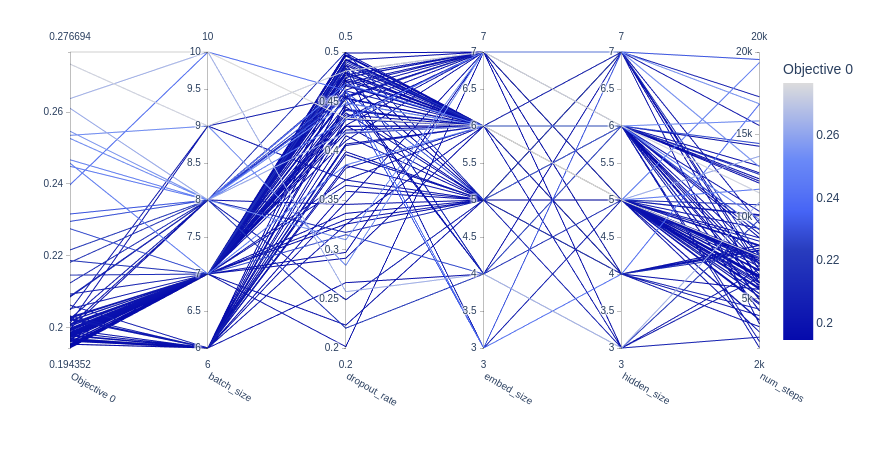
\includegraphics[scale=0.55]{./assets/optuna-params.png}
    \caption{Взаимосвязь параметров SGraphCM. Objective 0 -- цель оптимизации (бинарная кросс-энтропия на валидационном множестве). Более плотные и насыщенные линии указывают на более перспективные значения параметров.}
    \label{pic1}
\end{figure}

\newpage

\begin{figure}[ht]
    \centering
    \includesvg[width=0.75\textwidth]{./assets/valid_perplexity.svg}
    \caption{Зависимость перплексии от количества шагов на валидационном множестве.}
    \label{pic2}
\end{figure}

\begin{figure}[ht]
    \centering
    \includesvg[width=0.75\textwidth]{./assets/test_perplexity.svg}
    \caption{Зависимость перплексии от количества шагов на тестовом множестве.}
    \label{pic3}
\end{figure}

\newpage

\section{Алгоритм обогащения графа запросов}
\subsection{Об особенностях использования механизма внимания в графовых нейронных сетях}
\begin{figure}[ht]
\centering
\begin{minipage}{.5\textwidth}
  \centering
  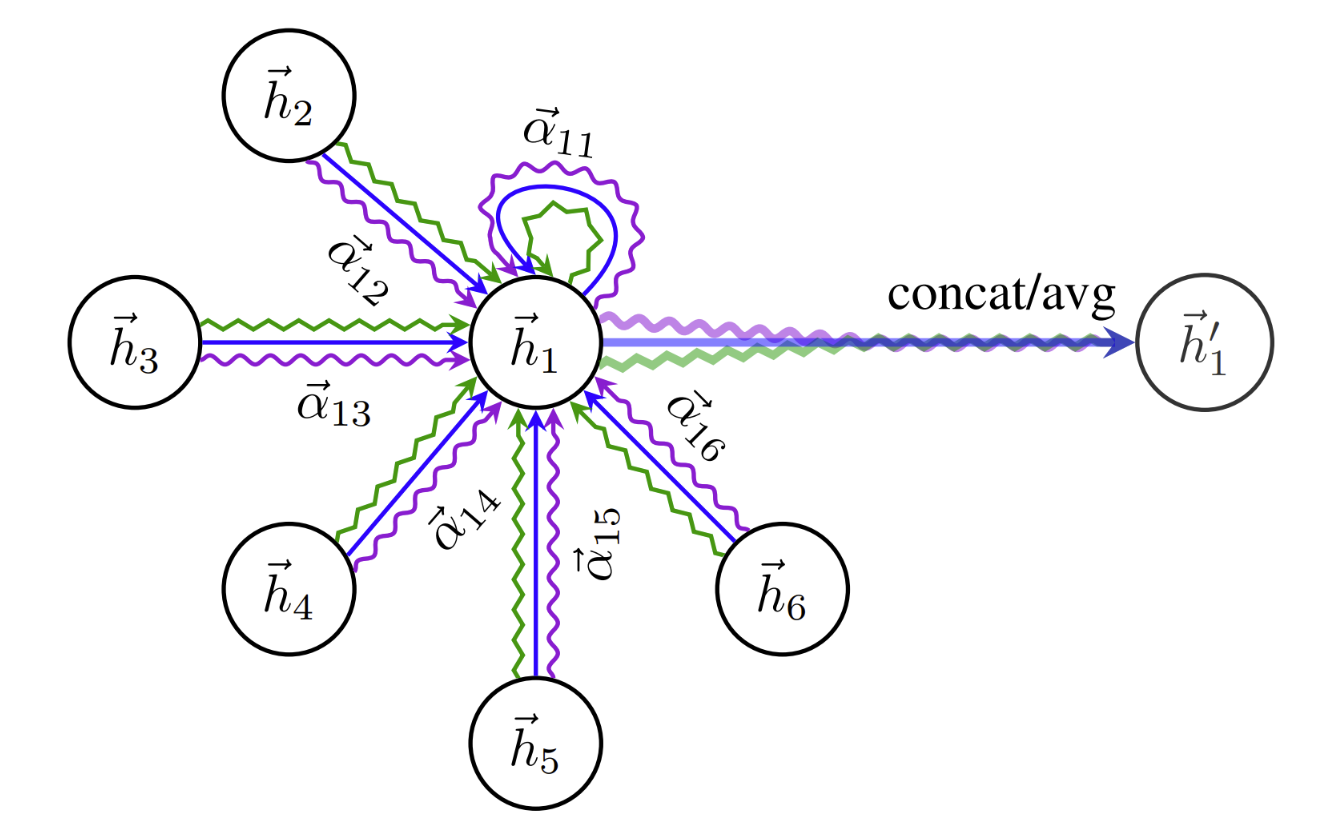
\includegraphics[width=1.0\linewidth]{./assets/GAT_layer_normal.png}
  \caption{Graph Attention}\label{pic4}
\end{minipage}%
\begin{minipage}{.5\textwidth}
  \centering
  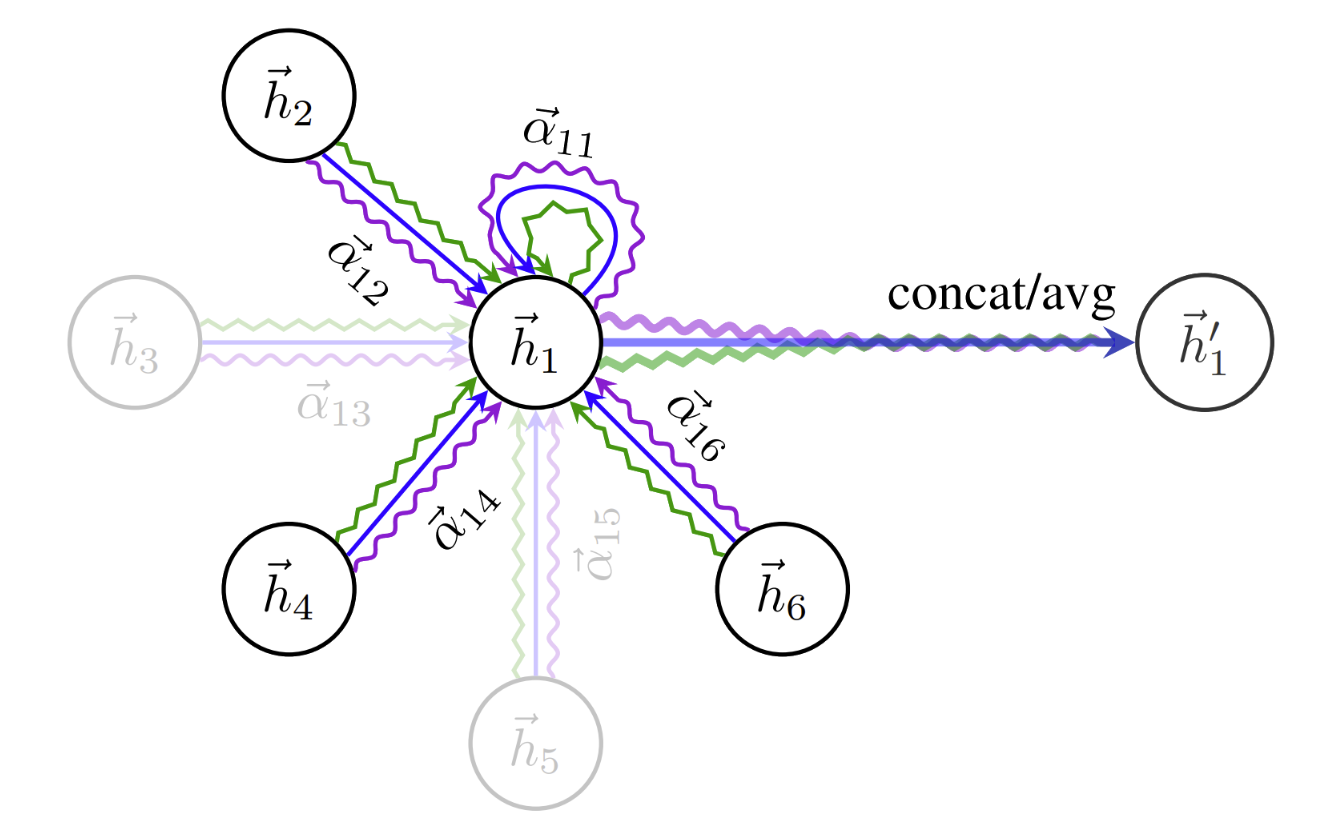
\includegraphics[width=1.0\linewidth]{./assets/GAT_layer_opacity.png}
  \caption{Graph Attention по подмножеству}\label{pic5}
\end{minipage}
\end{figure}

Рассмотрим подробнее слой механизма внимания для графов, изображенный на рис. \ref{pic4}, который задается формулой:
\begin{align}
    \vec{h}^{'}_i = \sigma \left( \frac{1}{K} \sum_{k=1}^K \sum_{j \in \mathcal{N}_i} \alpha_{ij}^k \mathbf{W}^k\vec{h}_j \right) \label{gat}
\end{align}
где, в случае для, например, графа запросов $\vec{h}_i^{'}$ -- итоговый эмбеддинг $i$-го запроса после применения операции, $\vec{h}_j$ -- эмбеддинги соседей до применения операции, $\mathcal{N}_i$ -- множество соседей $i$-го запроса, $\alpha_{ij}^k$ -- веса для механизма внимания соответствующих соседей, а $\mathbf{W}^k$ -- матрица весов слоя GAT.

На практике в графе могут существовать вершины с совершенно различным количеством соседей, как малым так и большим и, как следствие, данная операция может быть крайне затратна для ЭВМ в случае большого количества соседей. Для повышения стабильности обучения графовой модели широко распространен подход, который заключается в том, что в качестве соседей для вычисления GAT берётся лишь их некоторое подмножество соседей (рис. \ref{pic5}) в количестве не более чем $K$ штук. Для данной работы число соседей было выбрано $K=5$ исходя из относительно небольшого размера обучающей выборки.

Граф запросов строится по сессиям, а как мы знаем, один и тот же запрос $q$ может принадлежать нескольким различным сессиям ${s_{i_1}, \dots , s_{i_N}}$. Если предположить, что в сессиях $s_{i_1}, \dots , s_{i_n} : n < N$ были клики только в некоторый документ $d$, то это сформирует между соответствующими вершинами запросов ребра по правилу из 3.1. Однако сколько бы мы ни брали эквивалентных сессий (с таким же запросом и таким же кликнутым документом), это не добавит в граф ни новых вершин, ни новых ребёр, хотя интуитивно кажется, что эта информация могла бы быть полезна модели при обучении.

То есть граф запросов инвариантен к добавлению таких сессий, в которых встречается уже представленный в графе запрос и клик в документ по которому уже закодирован в виде ребра. Единственная возможность для модели использовать информацию о часто встречающихся запросах и документах это многократное обучение на тренировочных данных: в каждой эпохе обучения будут представлены все $n$ сессий с одинаковым запросом и одинаковым кликнутым документом, что ествественным образом даст представление о частотности запросов в сессиях.

Рассмотрим следующий алгоритм обогащения графа запросов информацией о соседях:
\begin{enumerate}
    [
    leftmargin=*,
    label={Шаг \arabic*.}
    ]
    \item Зададим нулем вес каждой вершины в графе запросов
    \item Для каждой сессии $s_i \in S$, для каждого кликнутого в ней документа $d_j \in D_i \in s_i : C_{ij} = 1$ прибавляем единицу к весу инцидентной ребру вершины, которая соответствует запросу $q_i \in s$.
    \item Каждое ненаправленное ребро заменим парой ориентированных ребёр с весами следующим образом: пусть ребро $e_{ij}$ инцидентно вершинам $v_i, v_k$, тогда добавим ребра $e_{ij}^{'}$ с весом вершины $v_j$ и ребро $e_{ji}^{'}$ с весом вершины $v_i$.
    \item Ненаправленные ребра и веса вершин удалим.
    \item Отнормируем веса исходящих из каждой вершины ребер: для каждой вершины $v_i$ новый вес ребра $e_{ij}$ равен $ w_{ij} = \frac{w_{ij}}{\sum_{q_k \in \mathcal{N}_i} w_{ik} }$, где $w_{ik}$ -- вес ребра $e_{ik}$
\end{enumerate}

Следует сделать замечание о случае, при котором существует несколько документов $d_{ij_{1}}, \dots , d_{ij_{m}}$, кликнутых по одному и тому же запросу $q_i$: вес соответствующей вершины увеличится на единицу столько раз, сколько по этому запросу $q_i$ было кликов суммарно во все эти документы.

Проиллюстрируем работу алгоритма на примере. Пусть по запросам $q_1, q_2$ были клики в один и тот же документ $d_1$ в количестве 4 и 10 раз соответственно, а по запросам $q_2, q_3$ в документ $d_2$ кликали 4 и 20 раз соответственно, в документ $d_3$ кликали 3 и 8 раз соответственно. Тогда без применения алгоритма граф запросов выглядел бы следующим образом: 
\begin{center}
\begin{tikzpicture}
    \SetUpEdge[lw         = 1.5pt,
        labelcolor = white]
    \GraphInit[vstyle=Normal]
    \SetGraphUnit{3}
    \tikzset{VertexStyle/.append  style={fill}}
    \Vertex[L=$q_1$]{1}
    \NOEA[L=$q_2$](1){2}
    \SOEA[L=$q_3$](2){3}
    \tikzset{EdgeStyle/.style={-}}
    \Edge(1)(2)
    \Edge(2)(3)
\end{tikzpicture}
\end{center}

После применения шагов 1 и 2 имеем:

\begin{center}
\begin{tikzpicture}
    \SetUpEdge[lw         = 1.5pt,
        labelcolor = white]
    \GraphInit[vstyle=Normal]
    \SetGraphUnit{3}
    \tikzset{VertexStyle/.append  style={fill}}
    \Vertex[L=$q_1$]{1}
    \node[above, yshift=0.4cm] at (1){4};
    \NOEA[L=$q_2$](1){2}
    \node[left, yshift=0.6cm] at (2){17=10+3+4};
    \SOEA[L=$q_3$](2){3}
    \node[above, yshift=0.6cm, xshift=0.2cm] at (3){28=20+8};
    \tikzset{EdgeStyle/.style={-}}
    \Edge(1)(2)
    \Edge(2)(3)
\end{tikzpicture}
\end{center}

Затем, после шагов 3 и 4:

\begin{center}
\begin{tikzpicture}
    \SetUpEdge[lw         = 1.5pt,
        labelcolor = white]
    \GraphInit[vstyle=Normal]
    \SetGraphUnit{3}
    \tikzset{VertexStyle/.append  style={fill}}
    \Vertex[L=$q_1$]{1}
    \NOEA[L=$q_2$](1){2}
    \SOEA[L=$q_3$](2){3}
    \tikzset{EdgeStyle/.style={->,relative=false,in=180,out=90}}
    \Edge[label=\text{$w_{12} = 17$}](1)(2)
    \tikzset{EdgeStyle/.style={->,relative=false,in=0,out=250}}
    \Edge[label=\text{$w_{21} = 4$}](2)(1)

    \tikzset{EdgeStyle/.style={->,relative=false,in=90,out=0}}
    \Edge[label=\text{$w_{23} = 28$}](2)(3)
    \tikzset{EdgeStyle/.style={->,relative=false,in=290,out=180}}
    \Edge[label=\text{$w_{32} = 17$}](3)(2)
\end{tikzpicture}
\end{center}

Веса после нормировки на шаге 5: $w_{12} = 1$, $w_{32} = 1$, $w_{21} = \frac{4}{32} = \frac{1}{8}$, $w_{23} = \frac{28}{32} = \frac{7}{8}$.

Модель, способную работать с таким взвешенным графом и сессиями в узком смысле будем называть SWGraphCM -- Simple Weighted Graph Click Model.

\subsection{Эксперимент}
Теперь если использовать веса ребер $w_{ij}$ в качестве вероятностей выбора соседа, то, в контексте примера, запрос $q_3$ будет чаще выбираться соседом для $q_2$ при обучении. Это приведет к тому, что модель будет чаще видеть, как мы предполагаем, более важного соседа и извлекать из этого нужную информацию раньше.

Применение данного алгоритма для графа запросов позволяет получать лучшее качество за меньшее число эпох (рис. \ref{pic6}). 

\begin{figure}[ht]
    \setcounter{figure}{5}
    % \centering
    \includesvg[width=1\textwidth]{./assets/weighted_vs_non.svg}
    \caption{Зависимость перплексии от количества шагов на тестовом множестве.}
    \label{pic6}
\end{figure}

Относительное улучшение, вычисленное как:
\begin{align}
    \frac{1}{N} \sum_{i=1}^{N} \frac{PPL_i^A - PPL_i^B}{PPL_i^A} \cdot 100\%
\end{align}
где $PPL^A$ -- перплексия модели с графом без модификаций, $PPL^B$ -- перплексия модели с обогащенным графом, составляет \textbf{19.16}\%. 

Стоит заметить, что если существует некоторый запрос $q_t$, попавший в проверочное множество, но не представленный в тренировочном, то использование одного графа запросов приведет к тому, что модель при обучении будет способна видеть данные, на которой будет проверяться её качество. Чтобы этого не произошло следует использовать два графа: тренировочный граф построенный только по тренировочным сессиями и проверочный, построенный по всем сессиям.

\section{Использование продолжительности просмотра документа}
Рассмотрим следующее поведение пользователя: в сессии $s$ по некоторому запросу $q$ он кликнул на документ $d_1$, расположенный на первой позиции, достаточно подробно его изучил и в целом был удовлетворен качеством поиска, однако решил изучить и другие найденные документы, например, кликнул в документ $d_2$, расположенный на второй позиции, но быстро понял, что содержимое его не удовлетворяет и закрыл документ. В результате модель на основе $DBN$ будет считать, что последний кликнутый документ $d_2$ более релевантен, потому что пользователь завершил на нем свою поисковую сессию, хотя в реальности мы имеем то, что более релевантным, очевидно, оказался документ $d_1$.

Таким образом, наша цель состоит в создании такой модели, которая, в описанном случае, давала бы оценку релевантности по запросу выше тому документу, который смотрели дольше. 

Избегать таких ложных результатов в оценках релевантности может метод $Clickrank$, поскольку в нем при достаточно большом времени просмотра документа соответствующий сомножитель $w_t$ нивелирует сомножитель порядка события в сессии $w_r$, однако он не является кликовой моделью. Мы же предлагаем добавить в кликовую модель на основе DBN события просмотра.

Пусть для каждого документа на позиции $j$ нам известно время $T_j$, на протяжении которого пользователь его изучал.

\subsection{Пороговая модель}
Простейшим вариантом работы со временем в нашем случае был бы выбор некоторого порога $\tau$, тогда мы могли бы рассматривать эквивалентные кликам события $V_j \in \{0, 1\}$, где $T_j > \tau \Rightarrow V_j = 1, иначе V_j = 0$. Однако, это не убережет от описанной проблемы, поскольку мы не можем измерять удовлетворенность, а значит, мы придем к тому же случаю -- если$\tau = 60$ секунд, документ $d_1$ смотрели час, а документ $d_2$ -- 2 минуты, то такая пороговая модель снова скажет, что документ $d_2$ более релевантен.

\subsection{Вероятностная модель}
Сделаем аналогичное $Clickrank$ предположение, что время просмотра документов распределено экспоненциально, т.е. имеем:
\begin{align}
    T_j = \left\{
        \begin{aligned}
            & X_j, & \text{где} \quad X_j \sim Exp(\lambda_u), \quad\textnormal{если}\quad A_j = 1 \quad\textnormal{и}\quad E_j = 1, \\
            & 0,  & \text{иначе} 
        \end{aligned}
        \right.
\end{align}

Также пусть удовлетворенность зависит от времени, т.е. уравнение (\ref{dbn:3}) теперь будет иметь вид
\begin{align}
    P(S_j=1 | T_j = t) = 1 - e^{-\beta_u t}
\end{align}

Такое задание зависимости согласуется с интуицией: если пользователь быстро прекратил изучение документа, то он его не удовлетворил. Обратно, чем больше времени пользователь изучает документ, тем более вероятно что он его удовлетворит.

Для использования модели необходимо найти вероятность удовлетворения документом при условии что пользователь его заметил и документ привлек его внимание:
\begin{align*}
    P(S_j = 1 | A_j = 1, E_j = 1) & = \mathbb{E}_{T_j}[1 - e^{-\beta_u T_j}] = \\
                                  & = \int_{0}^{+\infty} (1 - e^{-\beta_u t}) \lambda_u e^{-\lambda_u t} dt \\
                                  & = \int_{0}^{+\infty} \lambda_u e^{-\lambda_u t} dt - \lambda_u \int_{0}^{+\infty} e^{-(\beta_u + \lambda_u) t} dt \\
                                  & = 1 - \frac{\lambda_u}{\lambda_u + \beta_u} \\
                                  & = \frac{\beta_u}{\lambda_u + \beta_u}
\end{align*}

\textbf{Замечание.} Из свойств экспоненциального распределения имеем: $\mathbb{E}[T_u] = \frac{1}{\lambda_u} \Rightarrow \bar{T}_u = \frac{1}{\lambda_u}$.

Таким образом можно взять все исторические сессии по некоторому запросу $q$ и для каждого документа, который по этому запросу смотрели, посчитать среднее время просмотра и использовать в дальнейшем для предсказаний.

Привлекательность документ $a_u$ остается неизменной и вычисляется как для обычной модели на основе DBN с параметром $\gamma = 1$, а именно, как отношение количества кликов в документ $u$ к отношению показов данного документа не ниже последнего кликнутого документа.

Также, вместо параметра удовлетворительности документом $s_u$, у нас появляются два параметра: $\lambda_u$ и $\beta_u$. $\lambda_u$ отражает сколько времени пользователи проводят за изучением найденных поисковым алгоритмом документов. $\beta_u$ отвечает за то, насколько быстро документ способен удовлетворить пользователя.

Стоит сделать замечание, что мы будем придерживаться идентичной гипотезы, как в случае с кликами, т.е. будем считать удовлетворившим информационную потребность пользователя именно последний просмотренный документ. Мы делаем это исходя из того наблюдения, что хотя описанная ранее проблема может иметь место, она не массовая, поскольку DBN дает приемлемое качество и улучшает поисковую выдачу. Мы лишь хотим не так сильно пессимизировать кликнутые (или просмотренные) не последними документы. Из этого следует, что $1 - e^{-\beta_u t}$ -- удовлетворенность, а, соответственно, $e^{-\beta_u t}$ -- неудовлетворенность.

Данные новые параметры необходимо уметь оценивать, это можно сделать при помощи метода максимизации правдоподобия. Фукнция правдоподобия сессии $\mathcal{L}$ строится на основании действий пользователя с элементами выдачи следующим образом:

\begin{itemize}
    \item из гипотиз мы знаем, что пользователь может просмотреть лишь конечное число элементов на позициях $\{1, \dots, K\}$. Позицию последнего просмотренного документа для наглядности будем обозначать $K_i$, где $i$ -- индекс сессии $s_i$, которой принадлежит поисковая выдача. Пользователь проводит некоторое строго положительное время за изучением последнего документа, затем останавливается и сессия завершается. Из этого мы будем понимать, что, во-первых, документ на позиции $K_i$ был достаточно привлекателен, т.е. $A_{K_i} = 1$ и, во-вторых, оказался способен удовлетворить информационную потребность, т.е. $S_{K_i} = 1$. Вероятность этого равна $P(T_{K_i}, S_{K_i} = 1) = \underbrace{a_u}_{\text{привлекательность}} \cdot \underbrace{\lambda_u e^{-\lambda_u T_{K_i}}}_{\text{время просмотра}} \cdot \underbrace{(1 - e^{-\beta_u T_{K_i}})}_{\text{удовлетворенность}}$
    \item документы на позициях $j < K_i$ могли быть как просмотрены, так и не просмотрены. Если они были просмотрены, то они были достаточно привлекательными, но не удовлетворительными (в противном случае они были бы последними просмотренными). Значит, в случае просмотра $A_j = 1, S_j = 0$ и вероятность равна $P(T_j, S_j = 0) = a_u \cdot \lambda_u e^{-\lambda_u T_j} \cdot \underbrace{e^{-\beta_u T_j}}_{\text{неудовлетворенность}}$
    \item последний случай -- пользователь не был привлечен документом, тогда $T_j = 0$ и $P(T_j = 0) = 1 - a_u$.
\end{itemize}

В итоге имеем:
\begin{align}
    \mathcal{L}_i = \left( \prod_{j=1}^{K_i-1} \left[(1-a_u)\mathbb{I}_{[T_j=0]} + a_u \lambda_u e^{-(\lambda_u + \beta_u)T_j} \mathbb{I}_{[T_j > 0]} \right] \right) \cdot a_u \lambda_u e^{-\lambda_u T_{K_i}} (1 - e^{-\beta_u T_{K_i}})
\end{align}
и, соответственно
\begin{align}
    \ln\mathcal{L}_i = \sum_{j=1}^{K_i-1}\ln \left[ (1-a_u)\mathbb{I}_{[T_j=0]} + a_u \lambda_u e^{-(\lambda_u + \beta_u)T_j} \mathbb{I}_{[T_j > 0]} \right] + \ln(a_u\lambda_u e^{-\lambda_u T_{K_i}}) + \ln (1 - e^{-\beta_u T_{K_i}}) \label{mle:2}
\end{align}

Все сессии независимы в совокупности, это означает, что правдоподобие по всем сессиям равно $\mathcal{L} = \prod\limits_{i=1}^{N} \mathcal{L}_i \Rightarrow \ln \mathcal{L} = \sum\limits_{i=1}^{N} \ln \mathcal{L}_i$. 

\textbf{Замечание.} Поисковая выдача не содержит дублирующихся документов. Пусть нас интересует некоторый документ $u_{j_1}$. Документ не может быть одновременно просмотрен и не просмотрен, значит, в действительности под логарифмом будет только одно ненулевое слагаемое. Также этому документу будет соответствовать единственная позиция $j_1 < K_i$ в рамках поисковой выдачи -- документы на прочих позициях $u_{j \neq j_1}$ и их параметры $a_{u_j}, \lambda_{u_j}, \beta_{u_j}$ не будут зависеть от $u_{j_1}$ и в дальнейшем исчезнут при дифференцировании.    


Теперь получим оценки $\hat{a}_u, \hat{\lambda}_u, \hat{\beta}_u$. Как было замечено раньше, оценка $\hat{a}_u$ не поменяется в сравнении с классическим вариантом DBN, поскольку для нее у нас есть эквивалент события клика $T_j > 0 \Rightarrow C_j = 1$ и привлекательность документа никак не зависит от времени его просмотра -- просмотр начинается после клика. Тогда
\begin{align}
    \hat{a}_u = \frac{\sum\limits_{i=1}^{N}\mathbb{I}_{[C_u = 1]}}{\sum\limits_{i=1}^{N}\mathbb{I}_{[E_u = 1]}} 
\end{align}
где рассматриваются сессии по одинаковому запросу с интересующим нас документом $\{s_i\}_{i=1}^{N}$, а $C_u$ и $E_u$ это клик и показ документа $u$ в этих сессиях. Для интуитивного понимания можно сказать следующее: мы не будем рассматривать те сессии, где интересующий нас документ $u$ находился после последнего кликнутого документа, ведь в таком случае он точно никогда не был замечен и, соответственно, не мог быть кликнут. Тогда в знаменателе будет просто количество сессий, в которых документ $u$ гипотетически имел возможность быть кликнутым и в числителе количество кликов в него.

Оценка $\hat{\lambda}_u$ получается интереснее, но также не сложно: достаточно обратить внимание на два факта:
\begin{itemize}
    \item наблюдать проведенное за изучением документов время можно лишь в том случае, когда они точно были замечены и кликнуты
    \item при этом нас не интересует был ли пользователь удовлетворен документом, т.е. произошло ли завершение сессии
\end{itemize}

тогда из (\ref{mle:2}) пропадет $(1-a_u)\mathbb{I}_{[T_j=0]}$, а дифференцирование по $\lambda_u$ сократит все слагаемые, в которых $\lambda_u$ не представленно, а именно имеем следующие преобразования:

\begin{align}
    \ln\mathcal{L}_i = & \sum_{j=1}^{K_i-1} \left[ \ln(a_u) + \ln(\lambda_u) - \lambda_u T_j - \beta_u T_j \right] + \ln(a_u) + \ln(\lambda_u) - \lambda_u T_{K_i} + \ln(1-e^{-\beta_u T_{K_i}})
\end{align}

Последнее слагаемое не зависит от $\lambda_u$, а остальные могут быть добавлены под единый знак суммы, но теперь уже от $j=1$ до $K_i$. Вспомним, что для документа $u$ событие его просмотра имело место только на какой-то одной позиции. На других позициях были другие документы со своими параметрами, значит при дифференцировании они сократятся. Тогда если обозначить за $T_i^u$ время просмотра документа $u$ в сессии $s_i$, получим: 

\begin{align}
    \frac{\partial \ln \mathcal{L}}{\partial \lambda_u} = & \sum_{i=1}^{N} \left( \frac{\ln(\lambda_u) - \lambda_u T_i^u}{\partial \lambda_u} \right) = \frac{N}{\lambda_u} - \sum_{i=1}^{N}T_i^u = 0 \Rightarrow \hat{\lambda}_u = \frac{N}{\sum_{i=1}^{N}T_i^u}
\end{align}

Заметим сразу, что и $\hat{a}_u$ и $\hat{\lambda}_u$ могут вычисляться инкрементарно, т.е. при добавлении новой сессии в случае $\hat{a}_u$ необходимо будет безусловно прибавить единицу к знаменателю и если был клик, то ещё прибавить единицу к числителю. В случае $\hat{\lambda}_u$ необходимо будет прибавить к числителю единицу безусловно, а к знаменателю -- время просмотра документа $u$. Далее мы увидим, что для $\beta_u$ такие очевидные инкрементарные модификации будут невозможны.

Уравнение для оценки $\hat{\beta}_u$ получается из (\ref{mle:2}) аналогично, однако для наглядности рассмотрим производную логарифма правдоподобия для одной сессии из итоговой суммы:
\begin{align}
    \frac{\partial \ln \mathcal{L}_i}{\partial \beta_u} = -\sum_{j=1}^{K_i-1} T_j + \frac{T_{K_i} e^{-\beta_u T_{K_i}}}{1 - e^{-\beta_u T_{K_i}}} \label{grad:1}   
\end{align}

Первое слагаемое отвечает за событие просмотра документа, который был кликнут не последним. Второе слагаемое -- за последний просмотренный документ. Если документ был просмотрен в сессии, то он либо был последним просмотренным, либо не был таковым, соответственно, каждая сессия принесет либо $-T_i^u$, либо $\frac{T_i^u e^{-\beta_u T_i^u}}{1 - e^{-\beta_u T_i^u}}$. Тогда суммируя по всем сессиям имеем
\begin{align}
    \sum_{i \in \text{остановки}}\frac{T_i^u e^{-\beta_u T_i^u}}{1 - e^{-\beta_u T_i^u}} = \sum_{i \in \text{не остановки}} T_i^u
\end{align}

\textbf{Замечание.} Если документ достаточно редкий и у него есть только последний просмотр, то уравнение не имеет решения, поскольку $e^{-\beta_u T_j}$ не пересекает ноль. Тем не менее, из гипотиз следует, что такой документ должен считаться удовлетворительным, поэтому можно положить $\beta_u = +\infty$. Если по запросу таких уникальных документов с единственным просмотром несколько, то релевантность будет зависеть только от $a_u$ и в контексте примера, которым мы мотивировали использование просмотров, никаких улучшений не произойдет.

Чтобы решить поставленную задачу и добиться желаемого улучшения, мы будем полагать, что $\beta_u$ -- параметр зависящий от \textbf{запроса} и будем обозначать его $\beta_q$. Вид уравнения для $\beta$ не изменится -- каждая сессия сможет лишь добавить более одного слагаемого к правой части, т.е. в \textit{не остановках} теперь будет время \textit{всех} просмотренных не последними документов. 

\textbf{Мотивация.} Для каждого запроса можно установить некоторую ожидаемую продолжительность просмотра. Например, если пользователь желает найти фильм, то его длительность будет такой ожидаемой продолжительностью. Если пользователь ожидал найти более короткий документ, а ему предложены только длинные, то он не будет долго смотреть каждый, однако если среди них есть все же один короткий, то он посмотрит его дольше остальных и завершит сессию (поскольку это единственный такой документ и остальные для него априори нерелевантны). Тогда мы получим $\beta_q$, а уравнение, из которого мы сможем его получить, будет аналогично представленному ранее, с тем лишь отличием, что в суммах у нас будут принимать участие продолжительности просмотров всех документов. $\lambda_u$ же должен остаться уникальным для каждого документа.

Таким образом, если у нас будет оценка $\hat{\beta}_q$, зависящая только от запроса, две оценки $\hat{\lambda}_{d_{q,1}}, \hat{\lambda}_{d_{q,2}}$ для документов $d_{q,1}, d_{q,2}$ по этому запросу, то удовлетворительности этих документов будут различны: $\hat{\lambda}_{d_{q,1}} > \hat{\lambda}_{d_{q,2}} \Rightarrow s_{q,d_{q,1}} < s_{q,d_{q,2}}$ -- чем больше $\lambda$, тем меньше в среднем смотрели документ, и, по нашему предположению, меньше были удовлетворены.

Найти оптимальные оценки можно численно при помощи итерационных процессов, а именно метода Ньютона. Поскольку изначально мы хотим максимизировать функцию правдопобия, нам понадобится её градиент, который мы уже, по сути, вычислили: он имеет аналогичный (\ref{grad:1}) вид. Гессиан тогда равен
\begin{align}
    H(\beta_q) = - \sum_{\text{остановки}} \frac{(T_i^q)^2 e^{-\beta_q T_i^q}}{(1 - e^{-\beta_q T_i^q})^2}
\end{align}
Время просмотра не может быть отрицательным, для остановок оно должно быть строго положительным и легко видеть, что в таком случае $H(\beta_q) < 0$, следовательно функция правдоподобия строго вогнута и у нее существует единственный глобальный экстремум. Следовательно, уравнение $ f(\beta_q) = \frac{\partial \ln \mathcal{L}}{\partial \beta_q}$ имеет единственный корень, а $\frac{\partial f(\beta_q)}{\partial \beta_q} = H(\beta_q)$, тогда необходимо производить итерации:
\begin{align}
    \beta_q^{n+1} = \beta_q^{n} - \frac{f(\beta_q^n)}{H(\beta_q^n)}
\end{align}

В качестве начального приближения будем использовать $\beta_q^0 = \frac{1}{\sum\limits_{\text{остановки}} T_i^q}$ -- величину, обратную сумме продолжительностей просмотра всех последних просмотренных по данному запросу документов.

\subsection{Эксперимент}
Назовем описанную модель VSDBN -- View Simple Dynamic Bayesian Network \cite{vsdbn}.
Никакая модель библиотеки PyClick не работает со временем просмотра и, соответственно, игнориует соответствующее значение в исходных данных. Соответственно, первым этапом является подготовка данных. Имеющиеся сессии \cite{vkds} необходимо, во-первых, привести к пригодному для чтения PyClick формату и, во-вторых, подготовить хранилище сессий и их чтение к возможности сохранять время просмотра.

Время будем измерять в часах, поскольку время в секундах может быть слишком большим и при использовании экспонент приводить к существенным ошибкам при операциях с плавающей точкой или вовсе невозможность производить такие операции.

Будем считать $\beta_q$ с точностью до $\varepsilon = 10^{-6}$.

Для того чтобы посчитать перплексию по кликам, необходимо вывести вероятность клика в каждую позицию. Для первой позиции мы полагаем $P(E_1 = 1) = 1$, т.е. первый документ выдачи пользователь замечает гарантированно. Будет ли клик зависит в данном случае только от привлекательности, которая не меняется по сравнению с DBN.

Для позиций $j > 1$ необходимо учитывать удовлетворительность:
\begin{align}
    P(E_j = 1) = P(E_{j-1} = 1) \cdot \left[ \left(1 - \frac{\beta_q}{\beta_q + \lambda_{q,d_{j-1}}} \right) \cdot a_{q,d_{j-1}} + \left( 1 - a_{q,d_{j-1}} \right) \right] \label{exam:1}
\end{align}

-- пользователь увидит документ на позиции $j$ если документ на позиции $j-1$ не был привлекательным или он был привлекательным, но не был удовлетворительным. 

\subsubsection{Результат}

В таблице (\ref{table:results3}) приведены значения перплексии в таких же условиях, как для (\ref{table:results}). Модель SDBN имеет небольшое ухудшение по сравнию с DBN, поскольку используется $\gamma = 1$, в то время как для DBN параметр $\gamma$ оптимизировался.

Модель VSDBN имеет перплексию хуже, чем SDBN, но этот результат не может говорить о том, что модель хуже справляется с задачей, для которой она предназначается. Действительно, как видно из (\ref{exam:1}), наша модель может занижать вероятность для более поздних (с более старшими позициями в выдаче) кликов, поскольку если выше был долго просматриваемый документ, то вероятность того, что пользователь им был удовлетворен выше $\Rightarrow$ вероятность заметить более поздний докуменит ниже $\Rightarrow$ вероятность кликнуть в более поздний документ ниже, даже при том, что в действительности его могли смотреть, но недостаточно долго -- ровно для такого поведения пользователей и предлагается наша модель.

\begin{table}[ht]
    \centering
    \caption{Значение перплексии на идентичных наборах данных}
    \label{table:results3}
    \begin{tabular}{|l|l|}
        \thead{\bf Модель} & \thead{\bf PPL} \\
        \midrule\midrule
        SDBN                & \bf1.289           \\
        VSDBN & \underline{1.309} \\
        CTR            & 1.664 
    \end{tabular}
\end{table}

Качественно оценить результат работы модели можно на ранжировании: мы предполагаем, что наша модель должна давать оценку релевантности для документов с продолжительными просмотрами больше, чем с непродолжительными. Тогда если мы отсортируем документы по запросу по их оценкам релевантности, -- произведем переранжирование уже как-то отранжированной выдачи, -- мы ожидаем увидеть рост средней продолжительности просмотра первой позиции. 

\begin{table}[ht]
    \centering
    \caption{Средняя продолжительность просмотра первой позиции после переранжирования}
    \label{table:results4}
    \begin{tabular}{|l|l|}
        \thead{\bf Модель} & \thead{\bf{AvgViewTime} (в часах)} \\
        \midrule\midrule
        SDBN                & 1.090          \\
        VSDBN & \bf{\underline{1.269}} \\
        CTR            & 1.008 
    \end{tabular}
\end{table}

Таким образом видно, что применение нашей модели приводит к увеличению среднего времени просмотра документов на первой позиции на \textbf{16.42}\%, не сильно ухудшая вероятность кликов в выдачу в целом.


\chapter{Заключение}
В результате проведенных экспериментов удалось обучить модель GraphCM, работающую с сессиями в узком смысле, превосходящую по качеству классическую модель на основе DBN. Это достижение особенно примечательно, учитывая, что сессии в узком смысле не включают перезапросы и, следовательно, не предоставляют достаточной внутрисессионной информации. Несмотря на это ограничение, модель GraphCM смогла превзойти DBN, что демонстрирует её высокую эффективность и способность обрабатывать и анализировать данные даже в условиях ограниченной информации о взаимосвязи запросов. Эти результаты подчеркивают потенциал нейросетевых методов и их превосходство над традиционными подходами в задачах информационного поиска.

Также нам удалось предложить алгоритм для обогащения графа запросов информацией, применение которого позволяет тратить меньше ресурсов для обучения таких моделей. Более быстрое обучение способствует тому, что алгоритм ранжирования будет чаще обновляться, быстрее учитывать свежие данные и использовать их, предлагая пользователям более релевантные результаты.

Отступая от классических поведенческих сигналов, мы разработали модель VSDBN, учитывающую время просмотров документов для оценки их способности удовлетворять информационную потребность пользователей и, соответственно, релевантности, которая хотя и хуже DBN оценивает средние вероятноси кликов по документам в поисковой выдаче, но предлагает лучшие оценки релевантности в тех вертикалях поиска, где время просмотра играет существенную роль. 

В качестве направления для дальнейших исследований можно отметить следующее:
\begin{itemize}
    \item GraphCM не имеет модуля для оценки удовлетворительности документа, а результат её работы это вероятность клика, но не релевантность. Можно выделить отдельный модуль, отвечающий за удовлетворительность, который бы также учитывал не только клики, но и время просмотра, позволив объединить модели DBN и VSDBN и, вероятно, добиться лучшего качества по всем оцениваемым в работе параметрам
\end{itemize}


\begin{thebibliography}{00}
    \bibitem{clickrank}
    Guangyu Zhu and Gilad Mishne. 2012. ClickRank: Learning Session-Context Models to Enrich Web Search Ranking. ACM Trans. Web 6, 1, Article 1 (March 2012), 22 pages. https://doi.org/10.1145/2109205.2109206
    \bibitem{DBN}
    Olivier Chapelle and Ya Zhang. 2009. A dynamic bayesian network click model for web search ranking. In Proceedings of the 18th international conference on World wide web (WWW '09). Association for Computing Machinery, New York, NY, USA, 1-10. https://doi.org/10.1145/1526709.1526711
    \bibitem{GraphCM}
    Jianghao Lin, Weiwen Liu, Xinyi Dai, Weinan Zhang, Shuai Li, Ruiming Tang, Xiuqiang He, Jianye Hao, and Yong Yu. 2021. A Graph-Enhanced Click Model for Web Search. In Proceedings of the 44th International ACM SIGIR Conference on Research and Development in Information Retrieval (SIGIR '21). Association for Computing Machinery, New York, NY, USA, 1259-1268. https://doi.org/10.1145/3404835.3462895
    \bibitem{GAT}
    Veličković, P., Casanova, A., Liò, P., Cucurull, G., Romero, A., \& Bengio, Y. (2018). Graph attention networks. OpenReview.net. https://doi.org/10.17863/CAM.48429
    \bibitem{Attention}
    Ashish Vaswani, Noam Shazeer, Niki Parmar, Jakob Uszkoreit, Llion Jones, Aidan N. Gomez, Łukasz Kaiser, and Illia Polosukhin. 2017. Attention is all you need. In Proceedings of the 31st International Conference on Neural Information Processing Systems (NIPS'17). Curran Associates Inc., Red Hook, NY, USA, 6000-6010.
    \bibitem{GRU}
    Chung, J., Gulcehre, C., Cho, K., \& Bengio, Y. (2014). Empirical evaluation of gated recurrent neural networks on sequence modeling. In NIPS 2014 Workshop on Deep Learning, December 2014
    \bibitem{vkds}
    Информационный поиск, 2025. https://github.com/agcr/vk-ir-course, https://cloud.mail.ru/public/v332/zCGgiVD8c
    \bibitem{dbngithub}
    PyClick - Click Models for Web Search. https://github.com/markovi/PyClick/
    \bibitem{TianGong}
    Jia Chen, Jiaxin Mao, Yiqun Liu, Min Zhang, and Shaoping Ma. 2019. TianGong-ST: A New Dataset with Large-scale Refined Real-world Web Search Sessions. In Proceedings of the 28th ACM International Conference on Information and Knowledge Management (CIKM '19). Association for Computing Machinery, New York, NY, USA, 2485-2488. https://doi.org/10.1145/3357384.3358158
    \bibitem{vsdbn}
    View Simple Dynamic Bayesian Network. https://github.com/VictorDotZ/PyClick
\end{thebibliography}

\end{document}
